\documentclass[11pt]{article}

\usepackage[a4paper, margin=1in]{geometry}
\usepackage{mathtools}
\usepackage{outlines}
\usepackage{amsmath}
\usepackage{pdfpages}
\usepackage{verbatim}
\usepackage{listings}
\usepackage{algorithm}
\usepackage[noend]{algpseudocode}
% \usepackage[dvipsnames]{xcolor}
\usepackage[english]{babel}
\usepackage[labelfont=bf]{caption}
\usepackage{hyperref}
\usepackage{subcaption}
\usepackage{array}
\usepackage{longtable}
%\usepackage[T1]{fontenc}
\usepackage{titlesec, blindtext, color}
\usepackage{float}
\usepackage{xcolor}
\pagecolor{white}
\definecolor{gray75}{gray}{0.75}
\newcommand{\hsp}{\hspace{10pt}}
\titleformat{\section}[hang]{\Huge\bfseries}{\thesection\hsp\textcolor{gray75}{|}\hsp}{0pt}{\Huge\bfseries}

\captionsetup{labelfont=bf}

\makeatletter
\def\BState{\State\hskip-\ALG@thistlm}
\makeatother

\definecolor{codegreen}{rgb}{0,0.6,0}
\definecolor{codegray}{rgb}{0.5,0.5,0.5}
\definecolor{codepurple}{rgb}{0.58,0,0.82}
\definecolor{backcolour}{rgb}{0.95,0.95,0.95}


\lstdefinestyle{mystyle}{
    backgroundcolor=\color{backcolour},   
    commentstyle=\color{codegreen},
    keywordstyle=\color{blue},
    numberstyle=\tiny\color{codegray},
    stringstyle=\color{orange},
    basicstyle=\ttfamily\footnotesize,
    breakatwhitespace=false,         
    breaklines=true,                 
    captionpos=b,                    
    keepspaces=true,                 
    numbers=left,                    
    numbersep=5pt,                  
    showspaces=false,                
    showstringspaces=false,
    showtabs=false,                  
    tabsize=2
}

\lstset{style=mystyle}

\includeonly{
    chapters/Introduction,
    chapters/Agent,
    chapters/Rest,
    chapters/Antagonist,
    chapters/Dummy
}


\begin{document}
\begin{titlepage}
    \begin{center}
        \begin{figure}
            
\includegraphics[width=\textwidth]{img/marchio_unipi_pant541-eps-converted-to.pdf}         
        \end{figure}
        {\Large
        Artificial Intelligence and Data Engineering\\
        \vspace{5mm} %5mm vertical space
        Cloud Computing}\\
        \vspace{30mm} %5mm vertical space
        {\Huge\textbf{\textit{Docker Health Monitoring System}}}\\
        \vspace{10mm} %5mm vertical space
        {\Large Project Documentation}\\
        \par\noindent\rule{\textwidth}{0.4pt}
            \begin{flushright}
                \textit{TEAM MEMBERS}:\\
                Federica Baldi\\
                Daniele Cioffo\\
                Edoardo Fazzari\\ 
                Mirco Ramo\\
        	
            \end{flushright}
            \vfill
        Academic Year: 2020/2021\\        
    \end{center}
\end{titlepage} 
   
\tableofcontents

\section{Introduction}
The purpose of this project is to develop a system to monitor the health of a set of Docker hosts. The structure of such a system is as shown in the figure. 

\begin{figure}[H]
	\begin{subfigure}{\textwidth}
	\centering
		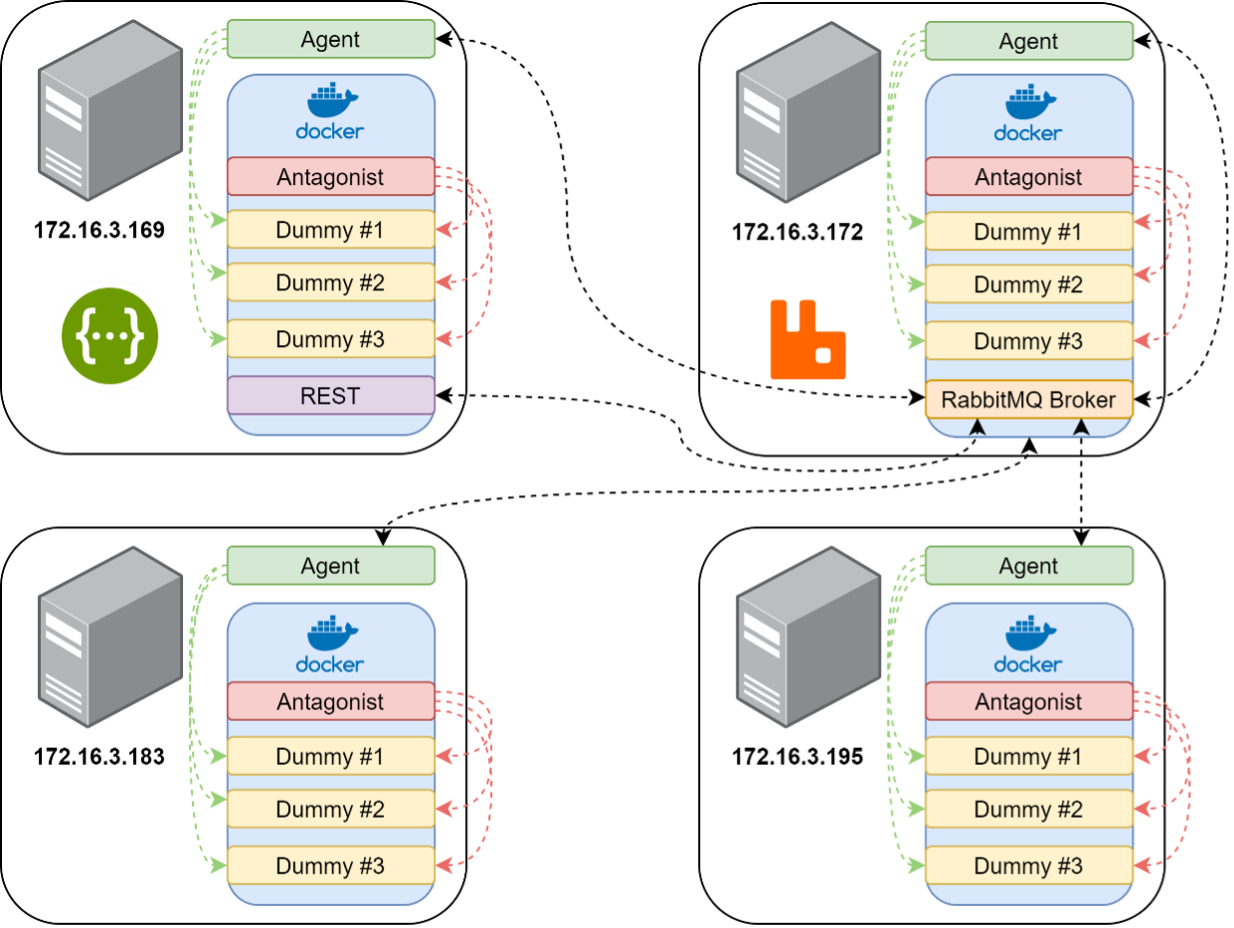
\includegraphics[width=0.9\linewidth]{img/structure.png} 
	\end{subfigure}
\end{figure}

\noindent On each Docker host runs an \textbf{agent}, a software whose task is to periodically check the wellbeing of containers running on the same host. Specifically, every x seconds the agent pings all containers in the \textit{"to be monitored"} list and calculates the experienced packet loss. If a container is down or if it is experiencing packet loss greater than a certain threshold, the agent must destroy it and automatically restart it. 

\noindent The list of containers to be monitored and the threshold are set by the system administrator, who communicates with the system via a \textbf{REST interface}. This interface is exposed by a control module running on one of the Docker hosts (in our case, on the machine with IP address 172.16.3.169).

\noindent In addition, one of the Docker hosts (in our case, the machine with IP address 172.16.3.172) exposes the \textbf{RabbitMQ broker service} as a container, thus allowing the various components (the agents and the swagger server to communicate.

\noindent To test the proper functioning of the system we have:
\begin{itemize}
	\item created "dummy" containers running on each Docker host that will be monitored by each of the agents 
	\item developed the \textbf{antagonist}, a small program running on each Docker host that periodically stops containers or artificially causes packet losses 
\end{itemize}
\section{Agent}
As already mentioned, the agent’s main task is to monitor the health of containers running on its same machine by pinging them periodically. The agent is nothing more than a Python program that can communicate with the Docker daemon thanks to the "docker" Python library\footnote{https://docker-py.readthedocs.io/en/stable/ }.

\noindent In order to talk to the Docker daemon, first of all a client is instantiated through the command \textit{from\_env()}. Then, the agent will start its periodic check.

\noindent Specifically, every \textit{INTERVAL\_BETWEEN\_PINGS} seconds, for each containers name in the \textit{MONITORED\_LIST} the agent performs the following actions:

\begin{itemize}
	\item It tries to retrieve the container object from its name. If the container does not exist on that particular host, the agent skips the next steps.
	\item It retrieves the IP address of the container within the bridge network. If the container has no IP address assigned, it means that it is not running, so the agent restarts it and skips the next steps.
	\item It pings the IP address of the container by sending 5 packets and it calculates the percentage of packet loss. If this percentage is higher than the \textit{THRESHOLD} value, then the agent restarts the container; otherwise, it assumes that everything is working properly.
\end{itemize}
In addition to the above actions, the agent also writes to a log file every time it performs a check or some action, so that it is easier for us to debug.

\noindent Moreover, in order to communicate with the other containers of the Health Monitoring System, the agent implements a \textbf{communication module} through which it receives the administration commands coming from the REST interface and forwarded by the relative \textbf{swagger server}, and performs the relative actions on all the monitored containers in the targeted hosts. (Of course every agent instance controls the host in which it runs).

\noindent To be precise, the \textbf{communication module subscribes} to different topics, corresponding to the possible commands that can be received by the administrator, and when a message is consumed, the body is decoded in order to perform the action. Those topics are:

\begin{enumerate}
	\item \textbf{threshold} (publisher: Swagger server, subscribers: agent instances, body: new\_value): asks to every receiver agent to change the allowed rate of packet loss for every monitored container
	\item \textbf{list\_request} (publisher: Swagger server, subscribers: agent instances, body: N/D): asks to every receiver agent the status of all the containers running in the target host, in terms of hostname, container name, operational status (running or exited) and monitoring status (monitored or non-monitored)
	\item textbf{actives} publisher: Swagger server, subscribers: agent instances, body: tuple(str hostname, str name, boolean new\_status): asks for a specific container to be added to (new\_status=True) or removed from (new\_status=False) the monitored list. Only the relative agent instance performs the action, the others discard the packet.
	\item \textbf{list\_response} (publishers: agent instances, subscriber: Swagger server, body: json\_str \textit{\[\{hostname: “hostname”, name: “name”, status: “running/exited”, monitored: ”true/false”\}\]}): response provided to list\_request, in which every agent instances report the status of the container running on the relative host
\end{enumerate}

\noindent Since the RabbitMQ consume operation is blocking, in order not to stale the agent we adopted the following solutions:
\begin{itemize}
	\item The communication module and the “pure agent” one run on \textbf{two different python threads}, in this way the administration command can still be received while the periodic check is performed
	\item The shared context is made only by two data structures, i.e.,  \textit{MONITORED\_LIST} and \textit{THRESHOLD} integer; every possible concurrent access to them has been avoided using the python explicit locking
	\item In order to minimize the lock time, instead of maintaining the lock for the entire agent’s read access to the shared variables, they are locally copied every time a periodic check is about to start, keeping the lock itself just for the copy time.
\end{itemize}


\section{REST Interface}
This REST APIs were generated using \textit{Swagger Editor} and the functionalities implemented are:

\begin{itemize}
	\item \textbf{GET}:
		\subitem \textit{containers/} : Retrieve the list of all containers with their informations. The \textit{response} is a list of containers containing for each one its hostname, its name, its status and if it is monitored or not.
	\item \textbf{POST}:
		\subitem \textit{containers/\{hostname\}/\{containerName\}} : Monitor container specified in the path
	\item \textbf{DELETE}:
		\subitem \textit{containers/\{hostname\}/\{containerName\}} : Unmonitor container specified in the path
	\item \textbf{PUT}:
		\subitem \textit{/threshold} : Update the packet loss threshold used in the Agent. The value is specified in the body of the request and its type is \textit{double}.
\end{itemize}

\noindent The REST Interface makes use also of a model for specifying the structure of a Container, which is the following\footnote{the asterisk indicates that the attribute must be set}:

\begin{figure}[H]
	\begin{subfigure}{\textwidth}
	\centering
		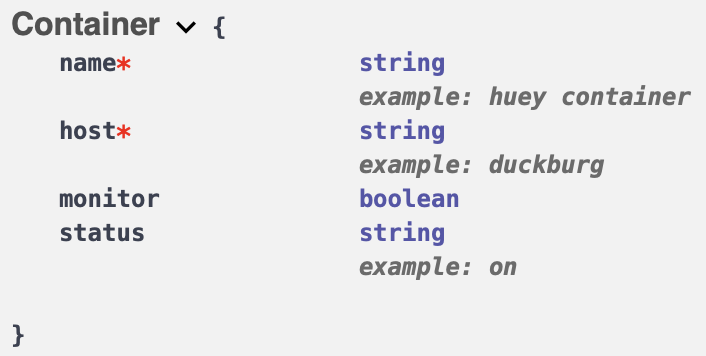
\includegraphics[width=0.9\linewidth]{img/container.png} 
	\end{subfigure}
\end{figure}
\section{Antagonist}
In order to test the health monitoring system a small program (the antagonist) has been developed to stop containers or cause some artificial packet loss.
More precisely, the antagonist was implemented in two different modules. 

\noindent One of the two modules is implemented in each host on a docker container, starting from a customized Ubuntu image. In this container there is the python interpreter which is used to execute the antagonist.py file.
This first module periodically attacks one of the local docker containers, simulating a stop of that container (leveraging the Docker API for python).

\noindent The second module has been implemented inside each dummy containers, which we will discuss in detail in the next chapter. This module allows you to simulate network problems on a certain container, through the use of the Netem library. The simulated packet loss percentage is periodically changed, through the use of this command: \emph{tc qdisc add dev eth0 root netem loss XX\%}, with XX the packet loss value.
\section{Dummy Container}
As already anticipated, in order to test the proper functioning of the system we created containers on each Docker host. These “dummy” containers are built from a custom image we created specifically for this project. In particular, it is an Ubuntu image that includes a Python interpreter and that runs two Python scripts at startup.

\noindent One of the two scripts is the actual dummy, and it is trivially an infinite loop that periodically prints messages specifying the time at which it was started and when it is being executed.

\noindent The other, as explained in the previous section, is the part of the antagonist that is responsible for creating artificial problems on the network.


\end{document}